% TikZ figure showing how blocks are splitted and encoded

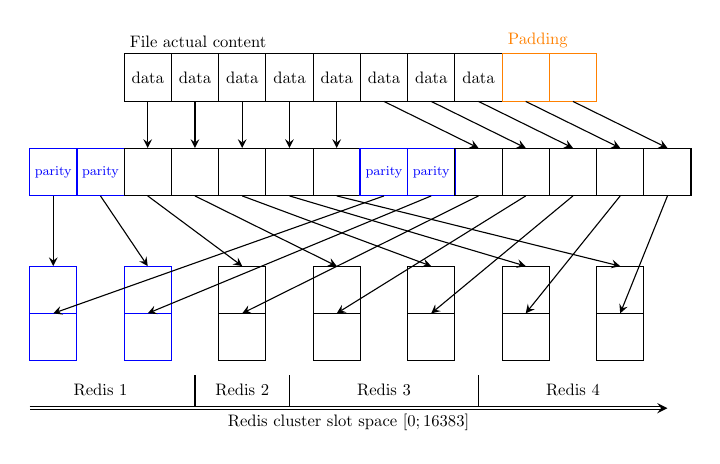
\begin{tikzpicture}[transform shape,scale=0.6]
\draw (1.5,0.5) node[above right] {File actual content};
\node (d1) at (2,0) [draw,minimum width=1cm,minimum height=1cm] {data};
\node (d2) at (3,0) [draw,minimum width=1cm,minimum height=1cm] {data};
\node (d3) at (4,0) [draw,minimum width=1cm,minimum height=1cm] {data};
\node (d4) at (5,0) [draw,minimum width=1cm,minimum height=1cm] {data};
\node (d5) at (6,0) [draw,minimum width=1cm,minimum height=1cm] {data};
\node (d6) at (7,0) [draw,minimum width=1cm,minimum height=1cm] {data};
\node (d7) at (8,0) [draw,minimum width=1cm,minimum height=1cm] {data};
\node (d8) at (9,0) [draw,minimum width=1cm,minimum height=1cm] {data};
\draw (9.5,0.5) node[above right,orange] {Padding};
\node (d9) at (10,0) [orange,draw,minimum width=1cm,minimum height=1cm] {};
\node (d10) at (11,0) [orange,draw,minimum width=1cm,minimum height=1cm] {};

\node (p1) at (0,-2) [draw,minimum width=1cm,minimum height=1cm,blue] {\footnotesize parity};
\node (p2) at (1,-2) [draw,minimum width=1cm,minimum height=1cm,blue] {\footnotesize parity};
\node (p3) at (2,-2) [draw,minimum width=1cm,minimum height=1cm] {};
\node (p4) at (3,-2) [draw,minimum width=1cm,minimum height=1cm] {};
\node (p5) at (4,-2) [draw,minimum width=1cm,minimum height=1cm] {};
\node (p6) at (5,-2) [draw,minimum width=1cm,minimum height=1cm] {};
\node (p7) at (6,-2) [draw,minimum width=1cm,minimum height=1cm] {};
\node (p8) at (7,-2) [draw,minimum width=1cm,minimum height=1cm,blue] {\footnotesize parity};
\node (p9) at (8,-2) [draw,minimum width=1cm,minimum height=1cm,blue] {\footnotesize parity};
\node (p10) at (9,-2) [draw,minimum width=1cm,minimum height=1cm] {};
\node (p11) at (10,-2) [draw,minimum width=1cm,minimum height=1cm] {};
\node (p12) at (11,-2) [draw,minimum width=1cm,minimum height=1cm] {};
\node (p13) at (12,-2) [draw,minimum width=1cm,minimum height=1cm] {};
\node (p14) at (13,-2) [draw,minimum width=1cm,minimum height=1cm] {};

\draw[->,>=stealth] (d1.south) to (p3.north);
\draw[->,>=stealth] (d2.south) to (p4.north);
\draw[->,>=stealth] (d3.south) to (p5.north);
\draw[->,>=stealth] (d4.south) to (p6.north);
\draw[->,>=stealth] (d5.south) to (p7.north);
\draw[->,>=stealth] (d6.south) to (p10.north);
\draw[->,>=stealth] (d7.south) to (p11.north);
\draw[->,>=stealth] (d8.south) to (p12.north);
\draw[->,>=stealth] (d9.south) to (p13.north);
\draw[->,>=stealth] (d10.south) to (p14.north);

\node (r1) at (0,-4.5) [blue,draw,minimum width=1cm,minimum height=1cm] {};
\node (r2) at (2,-4.5) [blue,draw,minimum width=1cm,minimum height=1cm] {};
\node (r3) at (4,-4.5) [draw,minimum width=1cm,minimum height=1cm] {};
\node (r4) at (6,-4.5) [draw,minimum width=1cm,minimum height=1cm] {};
\node (r5) at (8,-4.5) [draw,minimum width=1cm,minimum height=1cm] {};
\node (r6) at (10,-4.5) [draw,minimum width=1cm,minimum height=1cm] {};
\node (r7) at (12,-4.5) [draw,minimum width=1cm,minimum height=1cm] {};

\node (r8) at (0,-5.5) [blue,draw,minimum width=1cm,minimum height=1cm] {};
\node (r9) at (2,-5.5) [blue,draw,minimum width=1cm,minimum height=1cm] {};
\node (r10) at (4,-5.5) [draw,minimum width=1cm,minimum height=1cm] {};
\node (r11) at (6,-5.5) [draw,minimum width=1cm,minimum height=1cm] {};
\node (r12) at (8,-5.5) [draw,minimum width=1cm,minimum height=1cm] {};
\node (r13) at (10,-5.5) [draw,minimum width=1cm,minimum height=1cm] {};
\node (r14) at (12,-5.5) [draw,minimum width=1cm,minimum height=1cm] {};


\draw[->,>=stealth] (p1.south) to (r1.north);
\draw[->,>=stealth] (p2.south) to (r2.north);
\draw[->,>=stealth] (p3.south) to (r3.north);
\draw[->,>=stealth] (p4.south) to (r4.north);
\draw[->,>=stealth] (p5.south) to (r5.north);
\draw[->,>=stealth] (p6.south) to (r6.north);
\draw[->,>=stealth] (p7.south) to (r7.north);
\draw[->,>=stealth] (p8.south) to (r8.north);
\draw[->,>=stealth] (p9.south) to (r9.north);
\draw[->,>=stealth] (p10.south) to (r10.north);
\draw[->,>=stealth] (p11.south) to (r11.north);
\draw[->,>=stealth] (p12.south) to (r12.north);
\draw[->,>=stealth] (p13.south) to (r13.north);
\draw[->,>=stealth] (p14.south) to (r14.north);

\node (redis1) at (1,-6.6) {Redis 1};
\draw (3,-6.3) to (3,-6.95);
\node (redis1) at (4,-6.6) {Redis 2};
\draw (5,-6.3) to (5,-6.95);
\node (redis1) at (7,-6.6) {Redis 3};
\draw (9,-6.3) to (9,-6.95);
\node (redis1) at (11,-6.6) {Redis 4};
\draw[->,>=stealth,double] (-0.5,-7) to node[midway,below]{Redis cluster slot space $\left[0;16383\right]$} (13,-7);

\end{tikzpicture}
